 %----------------------------------------------------------------------------------------
%	PACKAGES AND OTHER DOCUMENT CONFIGURATIONS
%----------------------------------------------------------------------------------------

\documentclass[twoside]{article}

\usepackage{lipsum} % Package to generate dummy text throughout this template

\usepackage[sc]{mathpazo} % Use the Palatino font
\usepackage[T1]{fontenc} % Use 8-bit encoding that has 256 glyphs
\linespread{1.05} % Line spacing - Palatino needs more space between lines
\usepackage{microtype} % Slightly tweak font spacing for aesthetics

\usepackage[hmarginratio=1:1,top=32mm,columnsep=20pt]{geometry} % Document margins
\usepackage{multicol} % Used for the two-column layout of the document
\usepackage[hang, small,labelfont=bf,up,textfont=it,up]{caption} % Custom captions under/above floats in tables or figures
\usepackage{booktabs} % Horizontal rules in tables
\usepackage{float} % Required for tables and figures in the multi-column environment - they need to be placed in specific locations with the [H] (e.g. \begin{table}[H])
\usepackage{hyperref} % For hyperlinks in the PDF

\usepackage{lettrine} % The lettrine is the first enlarged letter at the beginning of the text
\usepackage{paralist} % Used for the compactitem environment which makes bullet points with less space between them

\usepackage{abstract} % Allows abstract customization
\renewcommand{\abstractnamefont}{\normalfont\bfseries} % Set the "Abstract" text to bold
\renewcommand{\abstracttextfont}{\normalfont\small\itshape} % Set the abstract itself to small italic text

\usepackage{titlesec} % Allows customization of titles
\renewcommand\thesection{\Roman{section}} % Roman numerals for the sections
\titleformat{\section}[block]{\large\scshape\centering}{\thesection.}{1em}{} % Change the look of the section titles
\titleformat{\subsection}[block]{\normalsize}{\thesubsection.}{1em}{} % Change the look of the section titles

\usepackage{fancyhdr} % Headers and footers
\pagestyle{fancy} % All pages have headers and footers
\fancyhead{} % Blank out the default header
\fancyfoot{} % Blank out the default footer
\fancyhead[C]{CA640 $\bullet$ 21/Nov/14 $\bullet$ Pr�cis Assignment} % Custom header text
\fancyfoot[RO,LE]{\thepage} % Custom footer text

\usepackage{natbib}
\bibliographystyle{agsm}

\usepackage{graphicx}
\usepackage{float}

\usepackage{setspace}

%----------------------------------------------------------------------------------------
%	TITLE SECTION
%----------------------------------------------------------------------------------------

\title{\vspace{-15mm}\fontsize{24pt}{10pt}\selectfont\textbf{Paper Pr�cis: Creating a Shared Understanding of Testing Culture on a Social Coding Site}} % Article title

\author{
\large
\textsc{Anthony Troy }\\[2mm] 
\normalsize \href{mailto:anthony.troy3@mail.dcu.ie}{anthony.troy3@mail.dcu.ie | 14212116} \\
\vspace{-5mm}
}
\date{}

%----------------------------------------------------------------------------------------

\begin{document}

\maketitle % Insert title

\thispagestyle{fancy} % All pages have headers and footers

%----------------------------------------------------------------------------------------
%	Disclaimer, Pr�cis & ABSTRACT
%----------------------------------------------------------------------------------------
\renewcommand{\abstractname}{\vspace{-\baselineskip}}
\begin{abstract}
\noindent \textbf{Disclaimer}: Submitted to Dublin City University, School of Computing for module CA640: Research Skills, 2014/2015. I hereby certify that the work presented and the material contained herein is my own except where explicitly stated references to other material are made.
\end{abstract}

\vspace{-7mm}

\renewcommand{\abstractname}{\vspace{-\baselineskip}}
\begin{abstract}
\noindent  \textbf{Basing Paper}: R. Pham, L. Singer, O. Liskin, F. Figueira Filho, and K. Schneider. Creating a shared understanding of testing culture on a social coding site. In Proceedings of the 2013 International Conference on Software Engineering, ICSE 2013, pages 112-121, Piscataway, NJ, USA, 2013. IEEE Press.
\end{abstract}

\vspace{1mm}
\renewcommand{\abstractname}{Abstract}
\begin{abstract}
\noindent 
Software engineering is inherently collaborative, at the team, project and community levels. However many project
owners battle with establishing and communicating a testing culture that is appropriate for their project's needs.
Transparent software environments such as Github incorporate social media features to make work more visible. 
Previous research forwards that this transparency influences the behaviour of developers. Our basing paper
extends upon those findings to investigate how the increased transparency found on GitHub influences testing 
behaviours.\par
From interviewing active GitHub users, both project owners and developers, our basing paper 
suggests several strategies that software teams can use to positively influence the testing behaviour in their projects. Additionally, it is found that project owners on GitHub are often not aware of these strategies. This research reports on the difficulties and risks which this causes and suggests guidelines for developing a sustainable testing culture.

\end{abstract}

%----------------------------------------------------------------------------------------
%	ARTICLE CONTENTS
%----------------------------------------------------------------------------------------

\begin{multicols}{2} % Two-column layout throughout the main article text

\section{Introduction}

Like many fields that rely closely on collaboration
and coordination, Software Engineering is rapidly transforming. The emergence of
social media sites --- both general and those specifically created for software 
developers --- has resulted in a paradigm shift in the field; developers 
can now connect with, provide help to, collaborate with, and learn from one another 
with ease \citep{Storey}. \par
By virtue social media sites provide a high degree of social transparency, 
making freely available the "social meta-data" around information exchange 
\citep{Stuart}. \citet{Dabbish} forwards that the transparency GitHub provides
influences the behaviour of software developers. Our basing paper investigates 
how testing behaviour is influenced by such social coding sites. \citet{Pham},
the paper author, poses that there exists no previous work on this topic and that
"if social coding sites can influence the testing behaviour of developers, they
might also have an impact on the progress of software development projects 
and their resulting projects". \par 
\setlength{\parskip}{0em} % hack 
This pr�cis is structured as follows. In section II, we describe some related works
around this topic, furthering from this section III outlines the respective study 
undertaken. Section IV and V discuss the emerged findings and section VI concludes 
this pr�cis.

%------------------------------------------------

\section{Related Work}
\par
\textbf{\textit{Testing Practices:}} a wealth of research has been conducted around
testing practices in OSS projects. For example, \citet{Michlmayr} conducted study 
that investigated the quality-related processes in a diverse set of open source projects. 
\citet{Greiler} specifically investigate testing practices in the Eclipse Plug-In community. 
\par

\textbf{\textit{Social coding sites}} have been subject to significant research efforts 
in recent years.
\citet{Stuart} forwards a conceptual framework on the effects of social 
transparency on behaviour. \citet{Singer} investigates "developer profile aggregators" 
that combine developer activities from social coding sites and other social media. 
\citet{Dabbish} explores the relationship between social transparency and developer 
behaviour on GitHub.
\par
While most of these studies report on concepts that are also found in our basing paper, 
Pham's contribution extends upon them by specifically exploring the related 
influences on testing.

%------------------------------------------------

\section{Study Design}

Our basing paper employs a general research method, Grounded Theory \citep{Anselm}, whereby two subject groups are analysed: project owners that receive pull requests (PRs) and contributors who send them.
\subsection{Research Questions}

For the initial data collection phase a survey was designed which included five questions to better help "understand how testing practices evolve based on the interaction between contributors and project owners on social coding sites" \citep{Pham}. This questionnaire (Q1) analysed the following topics:
\begin{itemize}
	\item how project owners assess incoming contributions
	\item internal and external motivations for engaging in testing efforts
	\item the challenges and risks related to testing
	\item how developers code with those challenges and risks
	\item	the impact of participating on social coding projects has on testing practices
\end{itemize} 

\subsection{Procedure}

Grounded Theory involves continuous data collection accompanied with periodic pauses for analysis. Accordingly, our basing study was conducted in three incremental phases of analysis. Pham first enlisted a diverse sample population though inviting active GitHub users belonging to popular OSS projects and random recently active users. The first phase sought to understand which testing-related norms and conventions exist on Github through asking participants to outline their testing process in one of their public projects. The findings here reflected that projects featuring extensive collaboration between developers demanded more elaborate testing approaches. They also indicated that most decisions regarding testing were made when PRs were sent and received, hence when people had to coordinate and negotiate their cooperation.
\par
Subsequently, the second phase of the analysis involved refining the target population to be "active users who used the collaboration features of GitHub" \citep{Pham}. Such was achieved by inviting the sample pool to take the first questionnaire (Q1), whereby the questionnaire responses made it possible to distinguish those users that had been collaboratively active and their approaches for testing. The refined target population were then invited to a round of semi-structured interviews exploring participant's testing practices and values. Several common themes emerged from these interviews:
\begin{enumerate}
	\item The social network features, fork and PR mechanisms, and integration of numerous tools result 		in a GitHub-specific process for sending and receiving contributions.
	\item GitHub tools and social features lower the barriers for engagement in software projects.
	\item GitHub integrates many tools into the project context and centralises many interactions and notifications among participants.
	\item GitHub provides increased social transparency that allows its users to see the identity, actions, and communications between users
\end{enumerate}
In the last phase, a final questionnaire (Q2) was sent to random GitHub users for quantitative validation of Pham's findings, this is outlined in section V.

%------------------------------------------------

\section{Findings}

\textbf{\textit{Interaction on GitHub with Regard to Testing:}} The interview process presented several common steps in the GitHub contribution process. After receiving a PR, a project owner manually reviews the contribution and assess it by different
aspects. Following such, they merged the PR into a testing branch and resolved conflicts manually. If a test suite existed, owners ran it to check whether or not this contribution passed. Finally, the contribution was merged into the main branch of the project. 
\par
It emerged that many factors that were taken into consideration by owners when assessing contributions, such are as follows: 
\begin{itemize}
\item \textbf{Contribution Size:} the perceived size of the changes highly influenced the project owner's need for tests.
\item \textbf{Developer Trust:} owners treated incoming PRs differently depending on whether they trusted the contributing developer.
\item \textbf{Contribution Type:} owners had different testing approaches for contributions that introduced a new feature and ones that changed existing code. The former were requested to include test whereas the latter caused project owners to check whether or not the changed code was already covered by existing tests. 
\end{itemize} 

\par
\textbf{\textit{Motivations for Demanding \& Delivering Tests:}} Owners had varied reasons for requiring tested contributions. According to one owner, maintaining clean and well documented code reduced the subsequent support effort. Some owners considered tests as a form of documentation of how to use the contributed feature. In another case, owners required acceptance-style tests to in turn communicate requirements. \par
In interviews with contributors, different motivations emerged for including tests in a PR. Some felt that explicitly adding tests highlighted the value of their contribution to the owner. Contributors identified existing tests in a project as informal project guidelines; thus feeling obligated to add their own tests. This obligation also appears from customs rooted in the community of the technology used. Ruby developers tested their contribution by default.

\textbf{\textit{Challenges and Risks:}} Interviewees saw an urgent need for automatic tests in their projects. They reported that many types of contributions needed to be managed and for reasons of scale could not be done using manual tests. In achieving automated testing, owners often saw it mandatory that a PR was to include respective tests. \citet{Pham} also discovered that projects who fail to "communicate testing culture efficiently and effectively", or who "set barriers that are too high for first-time contributors", will struggle to create and maintain a testing culture. For instance, if new contributors cannot easily find existing tests in a project, they will not be able to write any of their own. 
\par
Many owners expressed that their projects were struggling with creating the required testing culture, PRs received would often not include any tests by default. One issue they saw was the voluntary nature of OSS contributions: they could not simply require well-tested contributions. 

\textbf{\textit{Coping with Challenges:}} Scalability reasons drive owners towards automated tests, however manually merging each PR into a testing branch and running regression tests with a test suite of automated tests remained a tedious task. Many resorted to an automated continuous integration (CI) service, such as Travis CI or Jenkins. Freeing the owner of several manual steps: when a PR is received, a program merges the contribution into a testing branch, runs the existing test suite, and notifies the owner and contributor of the results.
\par
Owners developed varying processes around testing requirements and handling untested PRs. Due to the voluntary nature of GitHub, some owners simply resorted to writing tests themselves or thankfully requested further tests. Another approach was to lower the barriers and make it easier to provide tests. Other owners supplied access to learning resources and supported contributors who showed difficulties in writing tests.

\textbf{\textit{Impact of Social Coding Sites on Testing Practices:}} \citet{Pham} encountered different levels of lowering the effort for testing. One interviewee suggested that projects which use behaviour driven development (BDD) and concentrated on testing primarily the main use cases provided these low barriers to entry. A more extreme case of lowering the barrier for contributions was to defer testing to a later point. 
\par
Interviewees told us that effectively communicating a project's testing culture would lead to contributors adopting that culture more rapidly and in greater numbers. According some, better communication of testing culture leads to more PRs containing tests. Providing guidelines on contributing or dedicated testing tutorials removed uncertainties in contributors about how to participate correctly. Projects not communicating a testing culture often received PRs with no tests. 
\par
Central to owners creating and nurturing a testing culture is to supply existing tests and a simple testing infrastructure. Contributors reported this to lower the barrier, in turn increasing confidence in the correctness of their own code. Interviewees also argued that just having a test suite communicates certain values regarding testing, helping them understand the project's testing culture, norms, and conventions. 
\par
Since moving their projects to GitHub, interviewees reported that the number of volunteer contributions increased. They attributed this to the low barriers to entry and the resulting exposure to a larger number of developers. Many claimed that the public nature of GitHub results in improvements around testing practices. Some of these were "companies that used the exemplary testing practices in their public projects as an advertisement for the high quality of their development services". Similar was found in OSS projects, core members were concerned about the project's reputation and believed proper testing would lead to higher quality code, which in turn would be received better by others. One interviewee reported that having contributed to a high-profile project where tests are mandatory would help him find work.

\section{Validating Findings}
This section describes the striking results from the final questionnaire (Q2) which was used to validate core statements of Pham's findings. The according results are summarised in Table I, C  illustrates statements about contributors and PO about project owners. Each question presented participants with a Likert scale of five items ("I do not agree" to "I strongly agree"), such is represented in the diagrams on the X- axis with disagreement being on the left and agreement being on the right. The number of answers accumulated for each item is marked on the Y-axis.
\begin{table}[H]
  \centering
  	\caption{Result of final questionnaire (Q2)}
	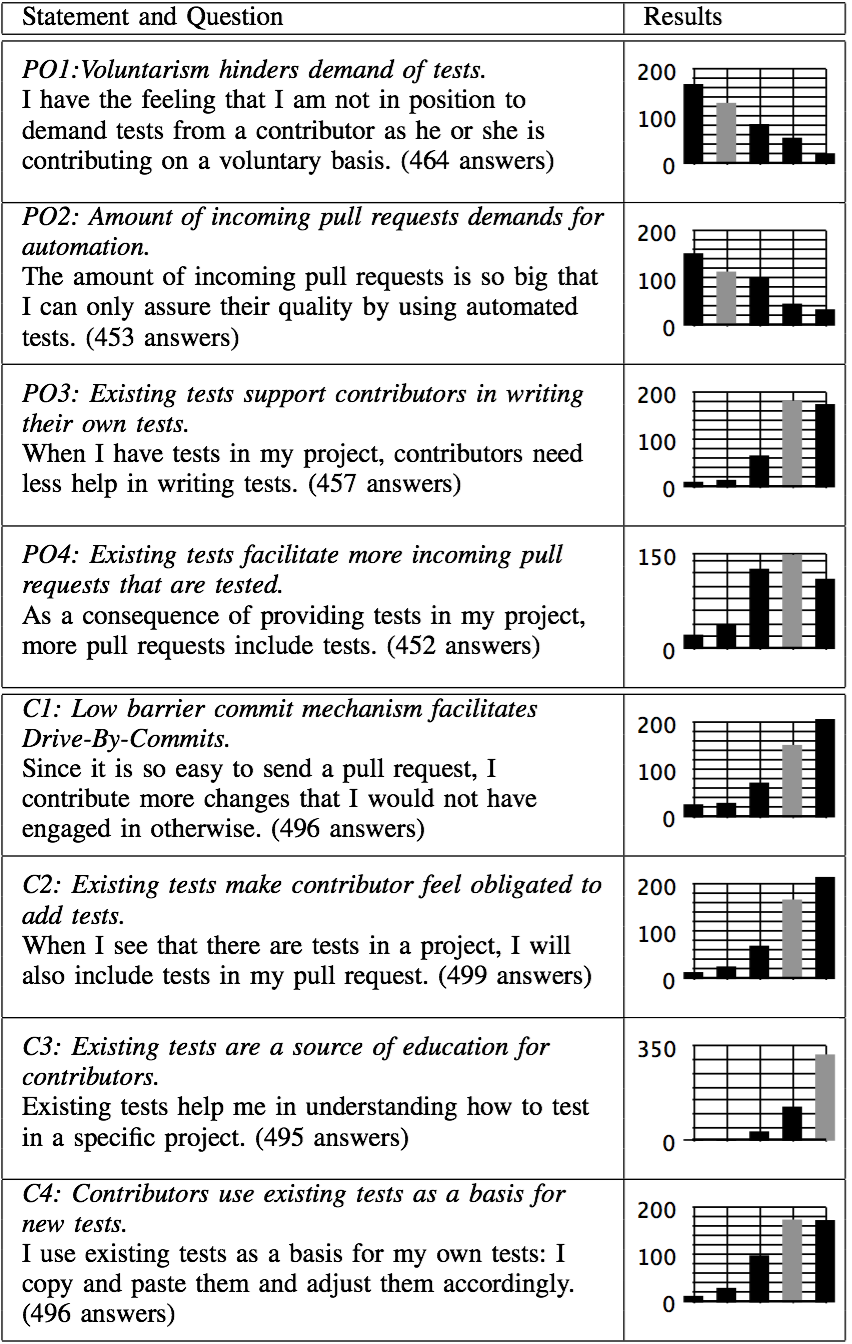
\includegraphics[width=77mm, height=150mm]{qa2.png}
\end{table}

As illustrated in Table 1, this questionnaire (Q2) yields some interesting responses. 
\begin{itemize}
\item modesty and humility of the requester as well as value given to the contribution may be influencing factors (PO1)
\item most participants did not agree to feel a need for automation (PO2)
\item owners agree that providing tests in one's project lowers the support effort regarding testing by contributors (PO3)
\item contributors heavily rely on existing test cases when creating their own, using them to learn how testing is done in a specific project (C3)
\item contributors copy existing tests and use them as a basis for new tests (C4)
\item contributors feel obligated to add their own tests and seem to comply with this implicit demand (C2).
\end{itemize} 

%------------------------------------------------

\section{Conclusions and Outlook} 

On social coding sites, project owners collaborate with contributors with varying ability and values regarding testing. Our basing paper reports on the influences of GitHub's peculiarities on testing practices --- particularly its high degree of social transparency, low barriers, and high degrees of integration and centralisation. Presented are insights around the contribution process on GitHub and how owners assess PRs with regard to testing. 
\par Developers on social coding sites can use Pham's findings to gain insights into issues contributors may face and the strategies that can be used to handle them. Software development organisations may take these contributions as inspiration for basing their own testing-related communication strategies on. This research is an exploratory first step to gain an understanding of the testing norms, challenges, and strategies on social coding sites. It is a starting point for informed, in-depth investigations into several of the issues raised.

%----------------------------------------------------------------------------------------
%	REFERENCE LIST
%----------------------------------------------------------------------------------------

\bibliography{article_2}

%----------------------------------------------------------------------------------------

\end{multicols}

\end{document}
